% Template taken with permission from Richard Hu
% Modified by Rahul Shah
% Last Updated: 2021-02-12 21:19

\documentclass[11pt]{article}
\usepackage{header}
\usepackage{mathrsfs}
\usepackage{mdframed}
\usepackage{pdfpages}
\usepackage{titlesec}

\newmdenv[%
    leftmargin=-5pt,
    rightmargin=-5pt, 
    innerleftmargin=5pt,
    innerrightmargin=5pt,
    backgroundcolor=brown!10,
]{Answer}%
\def\title{Homework 04}

\def\R{\mathbb{R}} % Real Numbers
\def\P{\mathbb{P}}
\def\A{\textbf{A}} % Bold matrices
\def\B{\textbf{B}}
\def\G{\textbf{G}}
\def\AB{\textbf{AB}}
\def\BA{\textbf{BA}}
\newcommand{\pd}[2]{\frac{\partial{#1}}{\partial{#2}}}
\let\originalmiddle=\middle
\def\middle#1{\mathrel{}\originalmiddle#1\mathrel{}}
\newcommand\aug{\fboxsep=-\fboxrule\!\!\!\fbox{\strut}\!\!\!}


\makeatletter
\newcount\my@repeat@count
\newcommand{\myrepeat}[2]{%
  \begingroup
  \my@repeat@count=\z@
  \@whilenum\my@repeat@count<#1\do{#2\advance\my@repeat@count\@ne}%
  \endgroup
}
\makeatother

\titlelabel{\thetitle.\enspace}


\begin{document}
\maketitle
\fontsize{12}{15}\selectfont

\begin{center}
	HW Due: February 19, 2021, at 23:59. \\
	Self-grades due: February 22, 2021, at 23:59.
\end{center}

\begin{enumerate}
	\item $\textbf{Reading Assignment}$
	      	              
	      For this homework, please review Note 5 and read Notes 6, 7. The notes 5 and 6 provide an overview of multiplication of matrices with vectors, by considering the example of water reservoirs and water pumps, and matrix inversion. Note 7 provides an introduction to vector spaces. You are always welcome and encouraged to read beyond this as well. Note 8 discusses column spaces and nullspaces, so it might be useful to read that for this homework as well.
	      	              
	      You have seen in Note 5 that the pump system can be represented by a state transition matrix. What constraint must this matrix satisfy in order for the pump system to obey water conservation?
	      \begin{Answer}
	      	The constraint is...
	      \end{Answer}
	      	      
	      	      
	      \newpage
	\item $\textbf{Feedback on your study group}$
	      	         
	      Please help us understand how your study groups are going! Fill out the following survey to help us create better matchings in the future. In case you have not been able to connect with a study group, or would like to try a new study group, there will be an opportunity for you to request a new study group as well in this form.
	      	             
	      \href{https://forms.gle/GAovoM3WxYYZYc5PA}{https://forms.gle/GAovoM3WxYYZYc5PA}
	      	             
	      To get full credit for this question you must (1) fill out the survey (it will record your email) and (2) indicate in your homework submission that you filled out the survey.
	      \begin{Answer}
	      	I did not fill out the survey
	      	% I filled out the survey!
	      \end{Answer}
	      	             
	      \newpage
	\item $\textbf{Mechanical Inverses}$
	      \begin{enumerate}[(a)]
	      	\item $\A = \begin{bmatrix}
	      	      0 & 1 \\
	      	      1 & 0
	      	\end{bmatrix}$
	      	\begin{enumerate}[i.]
	      		\item Find the inverse, $A^{-1}$, if it exists. If you find that the inverse does not exist, mention how you decided that. Solve this by hand.
	      		      \begin{Answer}
	      		      	Answer part a here
	      		      \end{Answer}
	      		\item \textbf{For parts (a)-(d),} in addition to finding the inverse (if it exists), describe how the matrix A transforms an arbitrary vector $\begin{bmatrix}
	      		      x \\
	      		      y
	      		\end{bmatrix}$.
	      			      		                    
	      		For example, if $\A \begin{bmatrix}
	      		x \\
	      		y
	      		\end{bmatrix} = \begin{bmatrix}
	      		2x \\
	      		2y
	      		\end{bmatrix}$, then $\A$ could scale $\begin{bmatrix}
	      		x \\
	      		y
	      		\end{bmatrix}$ by 2 to get $\begin{bmatrix}
	      		2x \\
	      		2y
	      		\end{bmatrix}$. If $\A \begin{bmatrix}
	      		x \\
	      		y
	      		\end{bmatrix}
	      		=
	      		\begin{bmatrix}
	      			x  \\
	      			-y 
	      		\end{bmatrix}$, then $\A$ could reflect $\begin{bmatrix}
	      		x \\
	      		y
	      		\end{bmatrix}$ across the x axis, etc. \textit{Hint: It may help to plot a few examples to recognize the pattern.}
	      		\begin{Answer}
	      			Answer part b here
	      		\end{Answer}
	      	\end{enumerate}
	      		      	               
	      	\newpage
	      	\item $\A = \begin{bmatrix}
	      	      -1 & 0 \\
	      	      0 & 1
	      	\end{bmatrix}$
	      	\begin{enumerate}[i.]
	      		\item Find the inverse, $A^{-1}$, if it exists. If you find that the inverse does not exist, mention how you decided that. Solve this by hand.
	      		      \begin{Answer}
	      		      	Answer part a here
	      		      \end{Answer}
	      		\item \textbf{For parts (a)-(d),} in addition to finding the inverse (if it exists), describe how the matrix A transforms an arbitrary vector $\begin{bmatrix}
	      		      x \\
	      		      y
	      		\end{bmatrix}$.
	      			      		                    
	      		For example, if $\A \begin{bmatrix}
	      		x \\
	      		y
	      		\end{bmatrix} = \begin{bmatrix}
	      		2x \\
	      		2y
	      		\end{bmatrix}$, then $\A$ could scale $\begin{bmatrix}
	      		x \\
	      		y
	      		\end{bmatrix}$ by 2 to get $\begin{bmatrix}
	      		2x \\
	      		2y
	      		\end{bmatrix}$. If $\A \begin{bmatrix}
	      		x \\
	      		y
	      		\end{bmatrix}
	      		=
	      		\begin{bmatrix}
	      			x  \\
	      			-y 
	      		\end{bmatrix}$, then $\A$ could reflect $\begin{bmatrix}
	      		x \\
	      		y
	      		\end{bmatrix}$ across the x axis, etc. \textit{Hint: It may help to plot a few examples to recognize the pattern.}
	      		\begin{Answer}
	      			Answer part b here
	      		\end{Answer}
	      	\end{enumerate}
	      		      	
	      		      		               
	      		      		                    
	      	\newpage
	      	\item $\A = \begin{bmatrix}
	      	      0 & 0 \\
	      	      0 & 1
	      	\end{bmatrix}$
	      		      		
	      	\begin{enumerate}[i.]
	      		\item Find the inverse, $A^{-1}$, if it exists. If you find that the inverse does not exist, mention how you decided that. Solve this by hand.
	      		      \begin{Answer}
	      		      	Answer part a here
	      		      \end{Answer}
	      		\item \textbf{For parts (a)-(d),} in addition to finding the inverse (if it exists), describe how the matrix A transforms an arbitrary vector $\begin{bmatrix}
	      		      x \\
	      		      y
	      		\end{bmatrix}$.
	      			      		                    
	      		For example, if $\A \begin{bmatrix}
	      		x \\
	      		y
	      		\end{bmatrix} = \begin{bmatrix}
	      		2x \\
	      		2y
	      		\end{bmatrix}$, then $\A$ could scale $\begin{bmatrix}
	      		x \\
	      		y
	      		\end{bmatrix}$ by 2 to get $\begin{bmatrix}
	      		2x \\
	      		2y
	      		\end{bmatrix}$. If $\A \begin{bmatrix}
	      		x \\
	      		y
	      		\end{bmatrix}
	      		=
	      		\begin{bmatrix}
	      			x  \\
	      			-y 
	      		\end{bmatrix}$, then $\A$ could reflect $\begin{bmatrix}
	      		x \\
	      		y
	      		\end{bmatrix}$ across the x axis, etc. \textit{Hint: It may help to plot a few examples to recognize the pattern.}
	      		\begin{Answer}
	      			Answer part b here
	      		\end{Answer}
	      	\end{enumerate}
	      	
	      	\newpage
	      	\item $\A = \begin{bmatrix}
	      	      \cos{\theta} & -\sin{\theta} \\
	      	      \sin{\theta} & \cos{\theta}
	      	\end{bmatrix}$
	      		      		                        
	      	Assume $\cos{\theta} \neq 0$. Hint: $\cos^2{\theta} + \sin^2{\theta} = 1$.
	      	\begin{enumerate}[i.]
	      		\item Find the inverse, $A^{-1}$, if it exists. If you find that the inverse does not exist, mention how you decided that. Solve this by hand.
	      		      \begin{Answer}
	      		      	Answer part a here
	      		      \end{Answer}
	      		\item \textbf{For parts (a)-(d),} in addition to finding the inverse (if it exists), describe how the matrix A transforms an arbitrary vector $\begin{bmatrix}
	      		      x \\
	      		      y
	      		\end{bmatrix}$.
	      			      		                    
	      		For example, if $\A \begin{bmatrix}
	      		x \\
	      		y
	      		\end{bmatrix} = \begin{bmatrix}
	      		2x \\
	      		2y
	      		\end{bmatrix}$, then $\A$ could scale $\begin{bmatrix}
	      		x \\
	      		y
	      		\end{bmatrix}$ by 2 to get $\begin{bmatrix}
	      		2x \\
	      		2y
	      		\end{bmatrix}$. If $\A \begin{bmatrix}
	      		x \\
	      		y
	      		\end{bmatrix}
	      		=
	      		\begin{bmatrix}
	      			x  \\
	      			-y 
	      		\end{bmatrix}$, then $\A$ could reflect $\begin{bmatrix}
	      		x \\
	      		y
	      		\end{bmatrix}$ across the x axis, etc. \textit{Hint: It may help to plot a few examples to recognize the pattern.}
	      		\begin{Answer}
	      			Answer part b here
	      		\end{Answer}
	      	\end{enumerate}
	      		      		                    
	      	\newpage
	      	\item $\A = \begin{bmatrix}
	      	      1 & 1 \\
	      	      2 & 0
	      	\end{bmatrix}$
	      	\begin{enumerate}[i.]
	      		\item Find the inverse, $A^{-1}$, if it exists. If you find that the inverse does not exist, mention how you decided that. Solve this by hand.
	      		      \begin{Answer}
	      		      	Answer part a here
	      		      \end{Answer}
	      		\item \textbf{For parts (a)-(d),} in addition to finding the inverse (if it exists), describe how the matrix A transforms an arbitrary vector $\begin{bmatrix}
	      		      x \\
	      		      y
	      		\end{bmatrix}$.
	      			      		                    
	      		For example, if $\A \begin{bmatrix}
	      		x \\
	      		y
	      		\end{bmatrix} = \begin{bmatrix}
	      		2x \\
	      		2y
	      		\end{bmatrix}$, then $\A$ could scale $\begin{bmatrix}
	      		x \\
	      		y
	      		\end{bmatrix}$ by 2 to get $\begin{bmatrix}
	      		2x \\
	      		2y
	      		\end{bmatrix}$. If $\A \begin{bmatrix}
	      		x \\
	      		y
	      		\end{bmatrix}
	      		=
	      		\begin{bmatrix}
	      			x  \\
	      			-y 
	      		\end{bmatrix}$, then $\A$ could reflect $\begin{bmatrix}
	      		x \\
	      		y
	      		\end{bmatrix}$ across the x axis, etc. \textit{Hint: It may help to plot a few examples to recognize the pattern.}
	      		\begin{Answer}
	      			Answer part b here
	      		\end{Answer}
	      	\end{enumerate}
	      		      		                    
	      	\newpage
	      	\item $\A = \begin{bmatrix}
	      	      1 & 0 & 0 \\
	      	      0 & 2 & 2 \\
	      	      1 & 4 & 4
	      	\end{bmatrix}$
	      	\begin{enumerate}[i.]
	      		\item Find the inverse, $A^{-1}$, if it exists. If you find that the inverse does not exist, mention how you decided that. Solve this by hand.
	      		      \begin{Answer}
	      		      	Answer part a here
	      		      \end{Answer}
	      		\item \textbf{For parts (a)-(d),} in addition to finding the inverse (if it exists), describe how the matrix A transforms an arbitrary vector $\begin{bmatrix}
	      		      x \\
	      		      y
	      		\end{bmatrix}$.
	      			      		                    
	      		For example, if $\A \begin{bmatrix}
	      		x \\
	      		y
	      		\end{bmatrix} = \begin{bmatrix}
	      		2x \\
	      		2y
	      		\end{bmatrix}$, then $\A$ could scale $\begin{bmatrix}
	      		x \\
	      		y
	      		\end{bmatrix}$ by 2 to get $\begin{bmatrix}
	      		2x \\
	      		2y
	      		\end{bmatrix}$. If $\A \begin{bmatrix}
	      		x \\
	      		y
	      		\end{bmatrix}
	      		=
	      		\begin{bmatrix}
	      			x  \\
	      			-y 
	      		\end{bmatrix}$, then $\A$ could reflect $\begin{bmatrix}
	      		x \\
	      		y
	      		\end{bmatrix}$ across the x axis, etc. \textit{Hint: It may help to plot a few examples to recognize the pattern.}
	      		\begin{Answer}
	      			Answer part b here
	      		\end{Answer}
	      	\end{enumerate}
	      \end{enumerate}
	      	      
	      \newpage
	\item $\textbf{Properties of Pump Systems}$
	      Throughout this problem, we will consider a system of reservoirs connected to each other through pumps.\\An example system is shown below in Figure 1, represented as a graph. Each node in the graph is marked with a letter and \textbf{represents a reservoir}. Each arrow in the graph represents a pump which moves a fraction of the water from one reservoir to the next at every time step. The \textbf{fraction of water} is written on top of the arrow.
	    \begin{figure}[h]
            \centering
            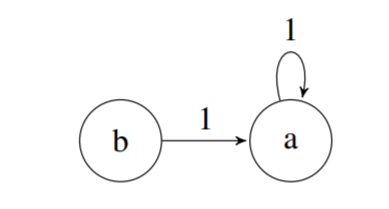
\includegraphics[scale=0.9]{q4a}
            \caption{ Pump system}
        \end{figure}
        
        For the system of pumps shown in Figure 1, find the associated state transition matrix. In other words, find the matrix A such that:
        \begin{enumerate}[(a)]
            \item For the system of pumps shown in Figure 1, find the associated state transition matrix. In other words, find the matrix A such that:
            \[
                \vec{x}[n+1] = \A\vec{x}[n],\text{ where }\vec x[n] = \begin{bmatrix}
                                                                        x_a[n] \\
                                                                        x_b[n]
                                                                      \end{bmatrix}
            \]
            $x_a[n]$ and $x_b[n]$ represent the amount of water in reservoir $a$ and $b$, respectively, at time step $n$.
            \begin{Answer}
                ..
            \end{Answer}
            
            \newpage
            
            \item Let us assume that at time step 0, the reservoirs are initialized to the following water levels: $x_a[0] = 0.5$, $x_b[0] = 0.5$. In a completely alternate universe, the reservoirs are initialized to the following water levels: $x_a[0] = 0.3, xb[0] = 0.7$. For both initial states, what are the water levels at timestep 1 $(\vec x[1])$?\\Use your answer from part (a) to compute your solution.
            \begin{Answer}
                ..
            \end{Answer}
            
            \newpage
            
            \item If you observe the reservoirs at timestep 1, i.e if you know $\vec x[1],$ can you figure out what the initial $(\vec x[0])$ water levels were? Why or why not?
            \begin{Answer}
                ..
            \end{Answer}
            
            \newpage
            
            \item Now let us generalize what we observed. Say there is a transition matrix $\A$ representing a pump system, and there exist two distinct initial state vectors/water levels: $\vec x_u[0]$ and $\vec x_v[0],$ that lead to the same state vector $\vec x[1]$ after $\A$ acts on them. You do not know which of the two initial state vectors you started in. Can you decide which initial state you started in by observing $\vec x[1]$? What does this say about the matrix $\A$?
            \begin{Answer}
                ..
            \end{Answer}
            
            \newpage
            
            \item Now, we want to prove the following theorem in a step-by-step fashion.\\Theorem: Consider a system consisting of k reservoirs such that the entries of each column in the system’s state transition matrix sum to one. If s is the total amount of water in the system at timestep $n$, then the total amount of water at timestep (n+1) will also be s.
            \begin{enumerate}[i.]
                \item 
Since the problem does not specify the transition matrix, let us start with a transition matrix
$\A = \begin{bmatrix}
        a_{11} & a_{12} \\
        a_{21} & a_{22}
    \end{bmatrix}$ and a state vector $\vec x[n] = \begin{bmatrix}
        x_1[n]\\
        x_2[n]
    \end{bmatrix}$ (this is an example when $k = 2$). In general, it is helpful to write as much out mathematically as you can in proofs. It can also be helpful to draw the transition graph. Write out what is “known”, i.e. ALL the information that is given to you in the theorem statement \textit{in mathematical form}.
    \begin{Answer}
        ..
    \end{Answer}
    \item Now write out what is to be proved \textit{in mathematical form}.
    \begin{Answer}
        ..
    \end{Answer}
    \item Prove the statement for the case of two reservoirs.
    \begin{Answer}
        ..
    \end{Answer}
    \item Now use what you learned to generalize to the case of $k$ reservoirs. \textit{Hint:} Think about $\A$ in terms of its columns, since you have information about sum of each column.
    \begin{Answer}
        ..
    \end{Answer}
            \end{enumerate}
            
            \newpage
            \item Set up the state transition matrix A for the system of pumps shown below. Compute the sum of the entries of each column of the state transition matrix. Are the sums greater than/less than/equal to 1?\\Explain what this A matrix physically implies about how the total amount of water in this system changes over time.
            
            \textit{Note:} If there is no “self-arrow/self-loop,” you can interpret it as a self-loop with weight 0, i.e. no water returns.
            \begin{figure}[h]
                \centering
                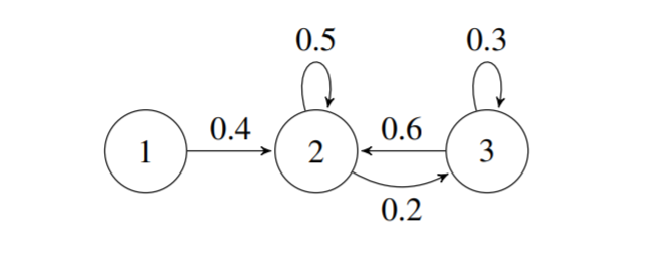
\includegraphics[scale=0.9]{q4f}
            \end{figure}
            \begin{Answer}
                ..
            \end{Answer}
        \end{enumerate}
	      \newpage
	      
	      \item OPTIONAL
	      \begin{Answer}
	           ...
	      \end{Answer}
	      
	      \newpage
	
	\item $\textbf{Finding Null Spaces and Column Spaces}$
	      \begin{enumerate}[(a)]
	      	\item Consider a matrix $\A \in \mathbb{R}^{3\times 5}$. What is the maximum possible number of linearly independent column vectors (i.e. the maximum possible dimension) of C($\A$)?
	      	\begin{Answer}
	      	      ...
	      	\end{Answer}
	      	
	      	\newpage
	      	
	      	\item You are given the following matrix $\A$
	      	\[
	      	    \A = \begin{bmatrix}
	      	        1 & 1 & 0 & -2 & 3 \\
	      	        0 & 0 & 1 & -1 & 1 \\
	      	        0 & 0 & 0 & 0 & 0
	      	    \end{bmatrix}
	      	\]
	        Find a \textit{minimum} set of vectors that span C($\A$) (i.e. a basis for C($\A$)). (This problem does not have a unique answer, since you can choose many different sets of vectors that fit the description here.) What is the dimension of C($\A$)?
	        
	        \textit{Hint: You can do this problem by observation. Alternatively, use Gaussian Elimination on the matrix to identify how many columns of the matrix are linearly independent. The columns with pivots (leading ones) in them correspond to the columns in the original matrix that are linearly independent}.
	        \begin{Answer}
	               ...
	        \end{Answer}
	        
	        \newpage
	        
	        \item Find a \textit{minimum} set of vectors that span N($\A$) (i.e. a basis for N($\A$)), where $\A$ is the same matrix as in part (b). What is the dimension of N($\A$)?
	        \begin{Answer}
	               ...
	        \end{Answer}
	        
            \newpage
            \item Find the sum of the dimensions of N($\A$) and C($\A$). What do you notice about this sum in relation to the dimensions of $\A$?
	        \begin{Answer}
	               ...
	        \end{Answer}
	        
	        \newpage
	        
	        \item Now consider the new matrix, $\B = \A^{T}, \begin{bmatrix}
	            1 & 0 & 0 \\
	            1 & 0 & 0 \\
	            0 & 1 & 0 \\
	            -2 & -1 & 0 \\
	            3 & 1 & 0
	        \end{bmatrix}$
	        Find a \textit{minimum} set of vectors that span C($\B$) (i.e. a basis for C($\B$)). What is the minimum number of vectors required to span the C($\B$)?
	        \begin{Answer}
	           ...
	        \end{Answer}
	        
	        
	        \newpage
	        
	        \item You are given the following matrix $\G$. Find a \textit{minimum} set of vectors that span N($\G$), i.e. a basis for N($\G$).
	        \[
	            \G = \begin{bmatrix}
	                2 & -4 & 4 & 8 \\
                    1 & -2 & 3 & 6 \\
                    2 & -4 & 5 & 10 \\
                    3 & -6 & 7 & 14
	            \end{bmatrix}
	        \]
	        \begin{Answer}
	           ...
	        \end{Answer}
	      \end{enumerate}
	      
	      \newpage
	      
	      \item OPTIONAL
	      	\begin{figure}[h]
                \centering
                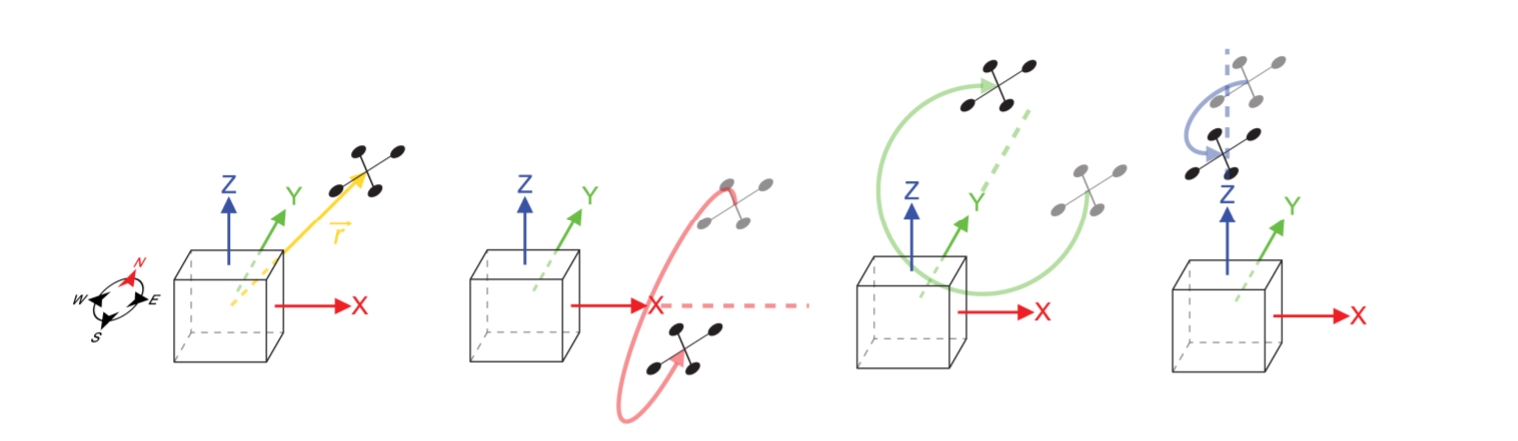
\includegraphics[scale=0.9]{q7a}
            \end{figure}
	      \begin{Answer}
	           ...
	      \end{Answer}
	      
	      
	      \newpage
	      
	\item $\textbf{Segway Tours}$
	      \begin{enumerate}
	      	\item Is it possible for the segway (essentially a stand on two wheels) to be brought upright and to a stop from any initial configuration? There is only one input (force) used to control two outputs (position and angle). You talk to a friend who is GSI'ing EE128, and she tells you that a segway can be modeled as a cart-pole system
	      	\begin{figure}[h]
                \centering
                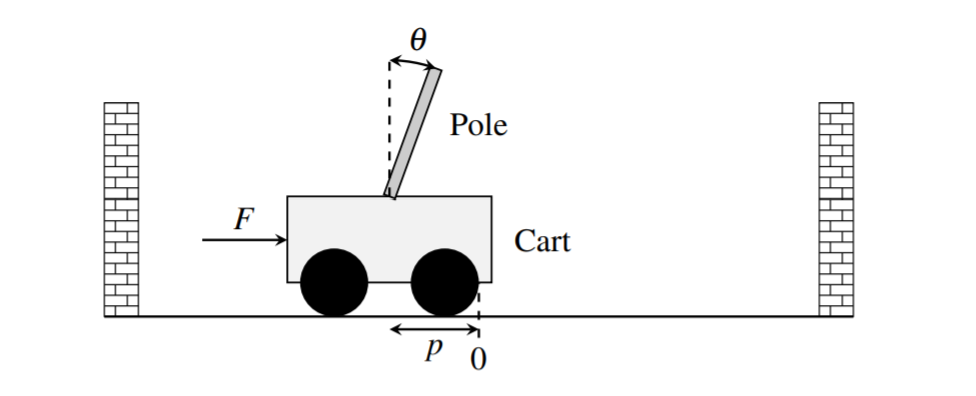
\includegraphics[scale=0.9]{q8a}
            \end{figure}
	      	
	      	A cart-pole system can be fully described by its position $p$, velocity $\dot p$, angle $\theta$, and angular velocity $\dot \theta$. We write this as a “state vector”, $\vec x = \begin{bmatrix}
                    p & \dot p & \theta & \dot \theta
	      	    \end{bmatrix}^T.$
	      	
	      	The input to this system is a scalar quantity $u[n]$ at time $n$, which is the force $F$ applied to the cart (or base of the segway). \footnote{You might note that velocity and angular velocity are derivatives of position and angle respectively. Differential equations are used to describe continuous time systems, which you will learn more about in EECS 16B. But even without these techniques, we can still approximate the solution to be a continuous time system by modeling it as a discrete time system where we take very small steps in time. We think about applying a force constantly for a given finite duration and we see how the system responds after that finite duration.}
	      	
	      	The cart-pole system can be represented by a linear model:
	      	\begin{equation}
	      	    \vec x[n+1] = \A\vec x[n] +\vec b_u[n],
	      	\end{equation}
	      	where $\A \in \R^{4\times4}$ and $\vec b \in \R^{4\times 1}$. Starting from some initial state $~\vec x_0$, can we reach a final desired state, $\vec x_f$, in $N$ steps?
	      	\begin{enumerate}[(a)]
	      	    \item Express $\vec{x}[1]$ ins terms of $\vec{x}[0]$ and the input $u[0]$.
	      	    \begin{Answer}
	      	        ...
	      	    \end{Answer}
	      	    
	      	    \newpage
	      	    
	      	    \item \begin{enumerate}[i.]
	      	        \item Express $\vec x[2]$ in terms of only $\vec x[0]$ and the inputs, $u[0]$ and $u[1]$.
	      	        \begin{Answer}
	      	            ...
	      	        \end{Answer}
	      	        
	      	        \vspace{10px}
	      	        \item Then express $\vec x[3]$ in terms of only $\vec x[0]$ and inputs $u[0]$, $u[1]$, and $u[2]$.
                    \begin{Answer}
	      	            ...
	      	        \end{Answer}
	      	        
	      	        \vspace{10px}
	      	        \item Finally express $\vec x[4]$ in terms of only $\vec x[0]$ and the inputs, $u[0], u[1], u[2]$, and $u[3]$.
                    
                    \textbf{Your expressions can have other relevant variables (e.g. A,~b etc) and mathematical operators.}
                    \begin{Answer}
	      	            ...
	      	        \end{Answer}
	      	    \end{enumerate}
	      	    
	      	    
	      	    \newpage
	      	    
	      	    \item Now, generalize the pattern you saw in the earlier part to write an expression for $\vec x[N]$ in terms of $\vec x[0]$ and the inputs from $u[0],\ldots ,u[N - 1]$. \textbf{Your expression can have other relevant variables (e.g. $\A$, $\vec b$ etc) and mathematical operators.}
	      	    
	      	    For the next four parts of the problem, you are given the matrix $\A$ and the vector $\vec b$: 
	      	    \[
	      	    A = \begin{bmatrix}
                    1 & 0.05 & -0.01 & 0 \\
                    0 & 0.22 & -0.17 & -0.01 \\
                    0 & 0.10 & 1.14 & 0.10 \\
                    0 & 1.66 & 2.85 & 1.14
	      	    \end{bmatrix}, \\  \vec b = \begin{bmatrix}
                                            0.01 \\
                                            0.21 \\
                                            -0.03 \\
                                            -0.44	      	    
	      	                            \end{bmatrix}
	      	    \]
	      	    Assume the cart-pole starts in an initial state $\vec x[0] = \begin{bmatrix}
	      	        -0.3853493 \\
                    6.1032227 \\
                    0.8120005 \\
                    -14
	      	    \end{bmatrix}$, and you want to reach the desired state $\vec x_f = \vec 0$ using the control inputs $u[0],u[1],\ldots$ etc. The state vector $\vec x_f =\vec 0$ corresponds to the cart-pole (or segway) being upright and stopped at the origin. \textbf{Reaching $\vec x_f =\vec 0$ in $N$ steps means that, given that we start at $\vec x[0]$, we can find control inputs ($u[0],u[1],\ldots$ etc), such that we get $\vec x[N]$ (i.e. state vector at $N$th time step) equal to $\vec x_f =\vec 0$.}
                    \begin{Answer}
	      	            ...
	      	        \end{Answer}
	      	    
	      	    % TODO: upload your own my_ipyntbk.pdf 
	      	% 	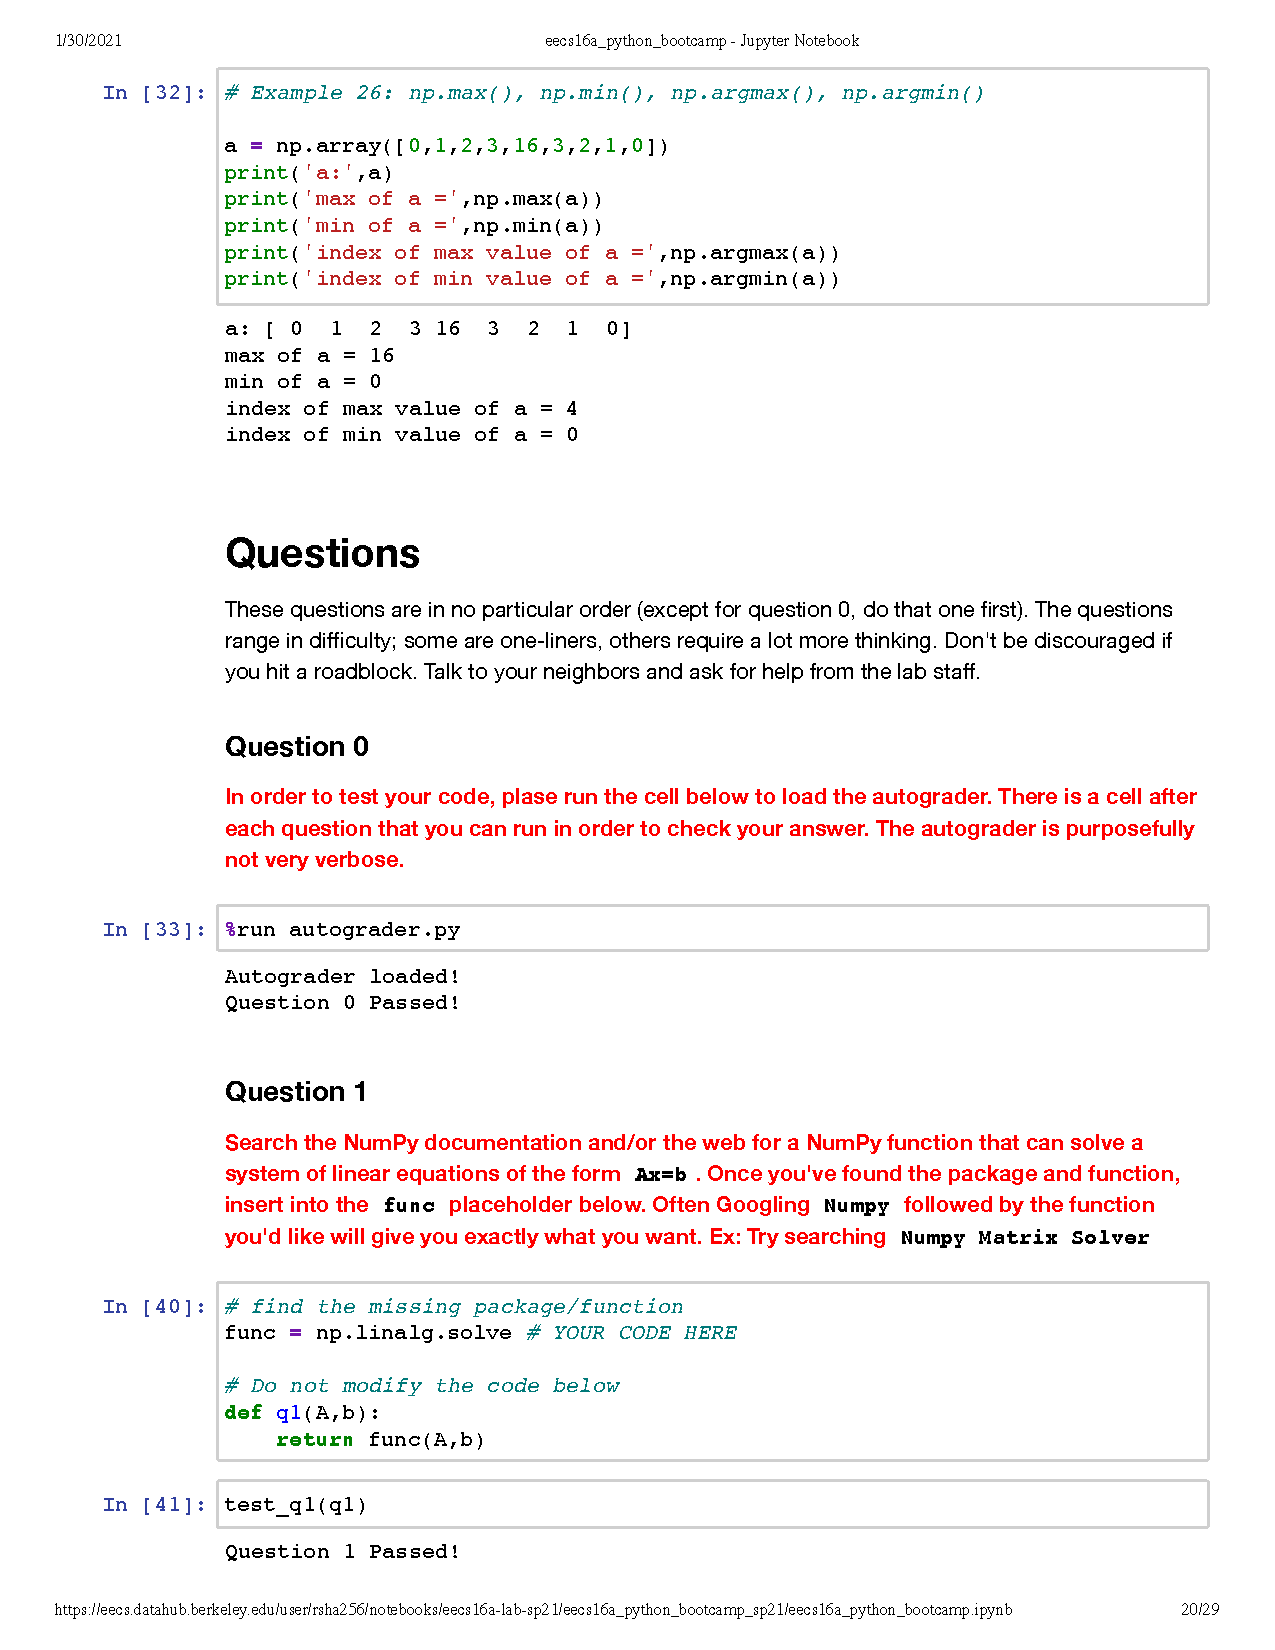
\includepdf[pages=-, noautoscale=true, scale=.8]{my_ipyntbk.pdf} 
	      		
	      		\newpage
	      	    \begin{Answer}
	      	            part h
	      	    \end{Answer}
	      	    
	      	    \newpage
	      	    \begin{Answer}
	      	            part i
	      	    \end{Answer}
	      	    
	      	\end{enumerate}

	      	
	      	
	      		\end{enumerate}
	      			      		   
	      		
	      			      		   
	      		\newpage
	      		\item $\textbf{Page Rank}$
	      		
	      		\begin{enumerate}
	      			\item For graph A shown below, what are the steady-state frequencies i.e. fraction of visitors in steadystate for the two webpages? Graph A has weights in place to help you construct the transition matrix.\\Remember to ensure that your steady state-frequencies sum to 1 to maintain conservation. 
	      			\begin{figure}[h]
                        \centering
                        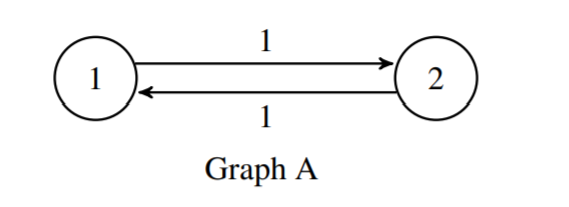
\includegraphics[scale=0.9]{q9a}
                    \end{figure}
	      			\begin{Answer}
	      				...
	      			\end{Answer}


                    \newpage
	      			\item For graph B, what are the steady-state frequencies for the webpages? You may use IPython and the Numpy command numpy.linalg.eig for this. It may be helpful to consult the \href{https://numpy.org/doc/stable/reference/generated/numpy.linalg.eig.html}{Python documentation} for numpy.linalg.eig to understand what this function does and what it returns. Graph B is shown below, with weights in place to help you construct the transition matrix.
	      			
	      			
    	      		\begin{figure}[h]
                            \centering
                            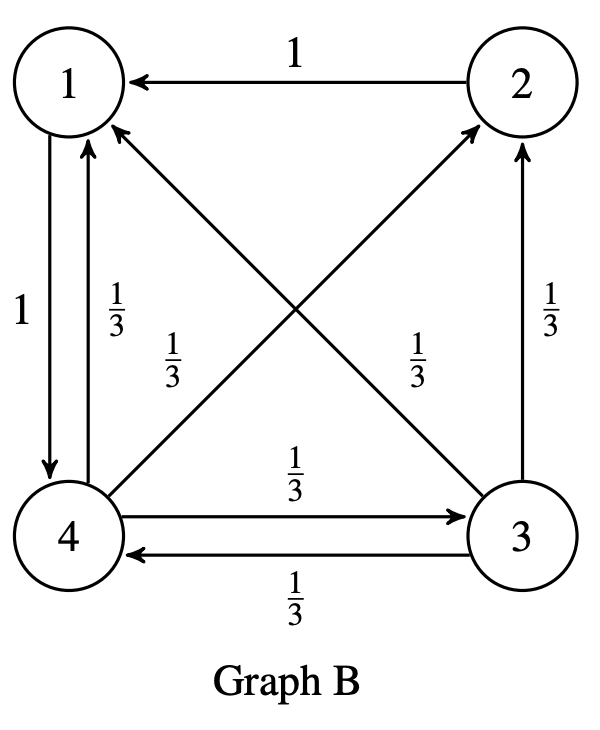
\includegraphics[scale=0.2]{q9b}
                    \end{figure}
      			      \begin{Answer}
      			      	...
      			      \end{Answer}
	      			      	      			          

                    \newpage
	      			\item Find the eigenspace that corresponds to the steady-state for graph C. How many independent systems (disjoint sets of webpages) are there in graph C versus in graph B? What is the dimension of the eigenspace corresponding to the steady-state for graph C? Again, graph C with weights in place is shown below. You may use IPython to compute the eigenvalues and eigenvectors again.
	      			\begin{figure}[h]
                        \centering
                        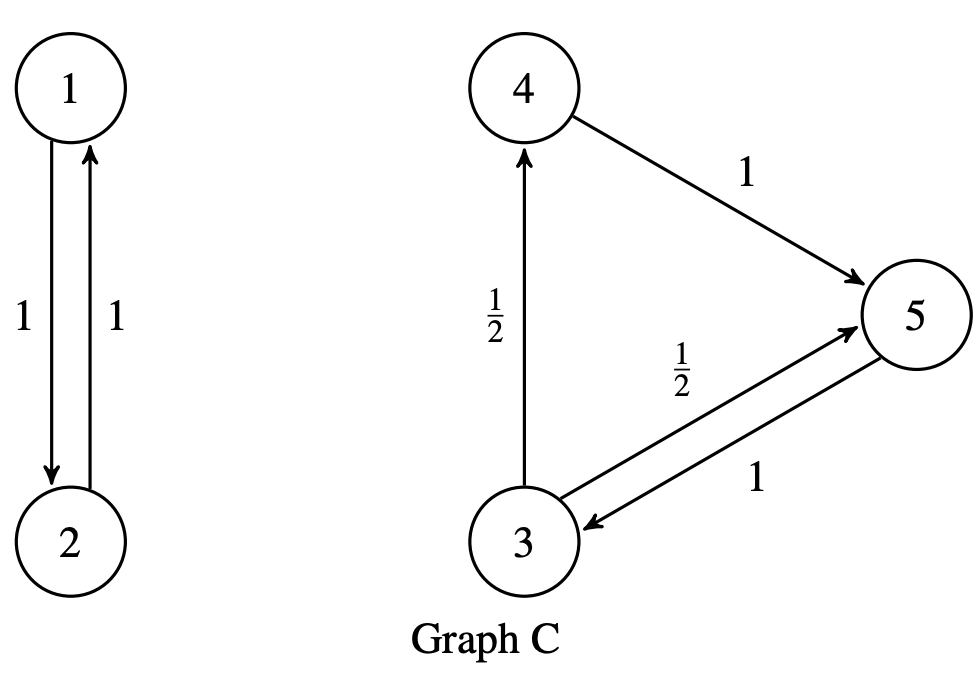
\includegraphics[scale=0.25]{q9c}
                    \end{figure}
      			      \begin{Answer}
      			      	...
      			      \end{Answer}
	      		\end{enumerate}
	      			      		   
	      			      		   
	      		\newpage
	      		\item $\textbf{Homework Process and Study Group}$
	      		Who did you work with on this homework? List names and student ID’s. (In case you met people at homework party or in office hours, you can also just describe the group.) How did you work on this homework? If you worked in your study group, explain what role each student played for the meetings this week.
	      			      		        
	      		\begin{Answer}
	      				      			            
	      		\end{Answer}
	      		\end{enumerate}
	      			      		
	      			      		
	      		\newpage
	      			      		
\end{document}
